\hypertarget{consideration-on-the-protocol-used-to-send-data-from-gps_android}{%
\subsection{Consideration on the protocol used to send data from
GPS\_Android}\label{consideration-on-the-protocol-used-to-send-data-from-gps_android}}

\hypertarget{description}{%
\subsubsection{Description}\label{description}}

During the group study solution design it became clear our system needs
\textbf{a mediator} which can control incoming messages. In particular:

\begin{itemize}
\tightlist
\item
  avoid loss of messages
\item
  provide the availability to many devices at once
\item
  provide smooth transmission to the processing subsystem
\end{itemize}

One of the initial requirements were to use UDP protocol.

\hypertarget{decision}{%
\subsubsection{Decision}\label{decision}}

First, we decided to \textbf{NOT} use UDP-based protocol, especially raw
UDP sockets:

\begin{itemize}
\tightlist
\item
  UDP connection are not reliable, you have to check the server receives
  messages correctly
\item
  Calculation of metrics may be very time- and resource-consuming, so we
  cannot afford to lose the result of works by message losing
\item
  A raw socket programmed software have to include additional checks,
  high-level integration is limited.
\end{itemize}

Therefore, we decided to use TCP-based protocols.

First, we used MQTT protocol because it well-suited for IoT-based
application. MQTT is useful for the reasons:

\begin{itemize}
\tightlist
\item
  fitting to criterion above
\item
  reliability
\item
  lightweight
\end{itemize}

\begin{figure}
\centering
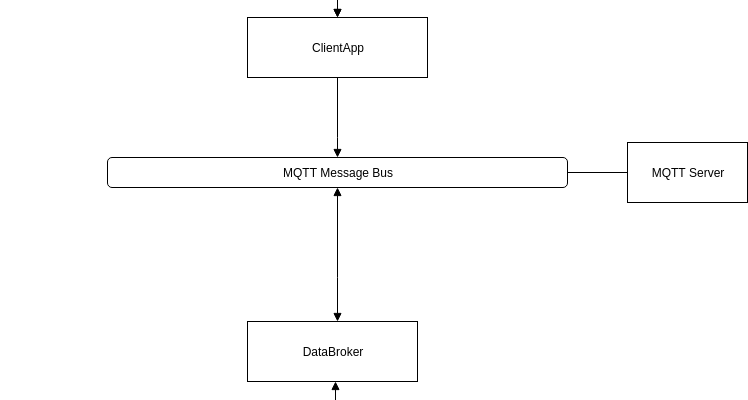
\includegraphics[width=0.5\textwidth,height=\textheight]{mqtt-justification.png}
\caption{mqtt-justification}
\end{figure}

However, the results in the first 3 experimental attempts have shown
that MQTT is not adapted for the system. Consequently, we switched to
HTTP protocol to send messages directly to backend server in
GPS\_Tracker.

\hypertarget{status}{%
\subsubsection{Status}\label{status}}

Accepted, corrected

\hypertarget{consequences}{%
\subsubsection{Consequences}\label{consequences}}

\begin{itemize}
\tightlist
\item
  A simple, supported and widely adapted protocol is used, further
  integration with TLS if needed
\item
  Possible additional overhead due to headers (can be solved in HTTP/2)
\end{itemize}

\hypertarget{consideration-on-the-protocol-used-to-send-data-from-gps_android-1}{%
\subsection{Consideration on the protocol used to send data from
GPS\_Android}\label{consideration-on-the-protocol-used-to-send-data-from-gps_android-1}}

\hypertarget{description-1}{%
\subsubsection{Description}\label{description-1}}

During the group study solution design it became clear our system needs
\textbf{a mediator} which can control incoming messages. In particular:

\begin{itemize}
\tightlist
\item
  avoid loss of messages
\item
  provide the availability to many devices at once
\item
  provide smooth transmission to the processing subsystem
\end{itemize}

One of the initial requirements were to use UDP protocol.

\hypertarget{decision-1}{%
\subsubsection{Decision}\label{decision-1}}

First, we decided to \textbf{NOT} use UDP-based protocol, especially raw
UDP sockets:

\begin{itemize}
\tightlist
\item
  UDP connection are not reliable, you have to check the server receives
  messages correctly
\item
  Calculation of metrics may be very time- and resource-consuming, so we
  cannot afford to lose the result of works by message losing
\item
  A raw socket programmed software have to include additional checks,
  high-level integration is limited.
\end{itemize}

Therefore, we decided to use TCP-based protocols.

First, we used MQTT protocol because it well-suited for IoT-based
application. MQTT is useful for the reasons:

\begin{itemize}
\tightlist
\item
  fitting to criterion above
\item
  reliability
\item
  lightweight
\end{itemize}

\begin{figure}
\centering
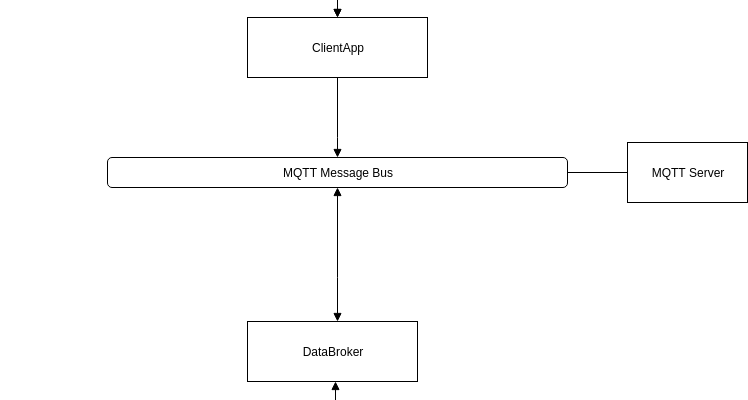
\includegraphics[width=0.5\textwidth,height=\textheight]{mqtt-justification.png}
\caption{mqtt-justification}
\end{figure}

However, the results in the first 3 experimental attempts have shown
that MQTT is not adapted for the system. Consequently, we switched to
HTTP protocol to send messages directly to backend server in
GPS\_Tracker.

\hypertarget{status-1}{%
\subsubsection{Status}\label{status-1}}

Accepted, corrected

\hypertarget{consequences-1}{%
\subsubsection{Consequences}\label{consequences-1}}

\begin{itemize}
\tightlist
\item
  A simple, supported and widely adapted protocol is used, further
  integration with TLS if needed
\item
  Possible additional overhead due to headers (can be solved in HTTP/2)
\end{itemize}
